\documentclass[tikz,border=7pt]{standalone}
\usepackage{iftex}
\ifPDFTeX
  \PackageError{matrix-figure}{This figure requires XeTeX or Tectonic}{Compile with xelatex or tectonic.}
\fi
\usepackage{fontspec}
\usepackage{xeCJK}
\usepackage{amsmath}
\usepackage{unicode-math}
\usepackage{xcolor}
\usepackage{tikz}
\usetikzlibrary{arrows.meta,positioning}

\providecommand{\FigureUseLocalFonts}{0}
\ifnum\FigureUseLocalFonts=1
  \setmainfont{NotoSansCJKtc-Regular.otf}[Path=\FigureSansFontPath]
  \setsansfont{NotoSansCJKtc-Regular.otf}[Path=\FigureSansFontPath,BoldFont=NotoSansCJKtc-Bold.otf]
  \setCJKmainfont{NotoSansCJKtc-Regular.otf}[Path=\FigureSansFontPath]
  \setCJKsansfont{NotoSansCJKtc-Regular.otf}[Path=\FigureSansFontPath,BoldFont=NotoSansCJKtc-Bold.otf]
  \setmathfont{STIXTwoMath.otf}[Path=\FigureMathFontPath]
\else
  \setmainfont{Noto Sans CJK TC}
  \setsansfont{Noto Sans CJK TC}
  \setCJKmainfont{Noto Sans CJK TC}
  \setCJKsansfont{Noto Sans CJK TC}
  \setmathfont{STIX Two Math}
\fi

\definecolor{FigureInk}{HTML}{253142}
\definecolor{PanelFill}{gray}{0.96}
\definecolor{RowShade}{gray}{0.86}
\definecolor{ColumnShade}{gray}{0.74}
\definecolor{ResultShade}{gray}{0.58}
\definecolor{FocusShade}{gray}{0.68}
\definecolor{GuideShade}{gray}{0.80}

\newcommand{\MatrixCell}[2]{%
  \tikz[baseline=(value.base)]{\node[fill=#1,rounded corners=0.4pt,inner sep=2.2pt,
    minimum width=1.35em,minimum height=1.35em] (value) {$#2$};}%
}
\newcommand{\RowCell}[1]{\MatrixCell{RowShade}{#1}}
\newcommand{\ColumnCell}[1]{\MatrixCell{ColumnShade}{#1}}
\newcommand{\ResultCell}[1]{\MatrixCell{ResultShade}{#1}}
\newcommand{\FocusCell}[1]{\MatrixCell{FocusShade}{#1}}

\tikzset{
  figure/.style={font=\sffamily,text=FigureInk,>={Stealth[length=3.5mm,width=2.5mm]}},
  panel/.style={draw=FigureInk,line width=0.9pt,rounded corners=1.5mm,fill=PanelFill,align=center},
  flow/.style={-{Stealth},line width=1.05pt,draw=FigureInk},
}


\begin{document}
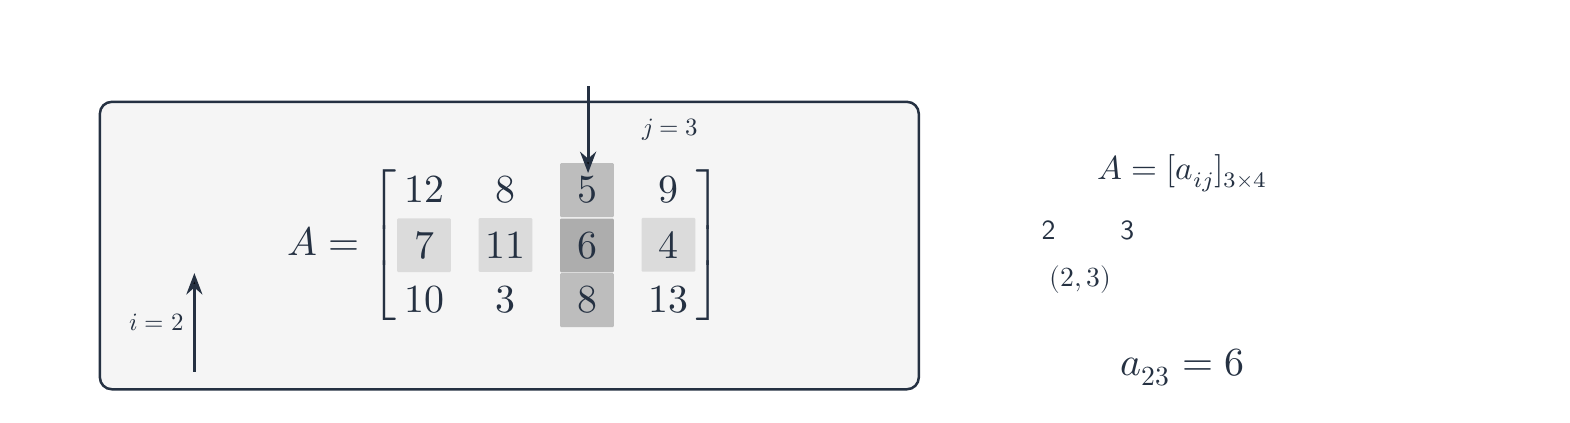
\begin{tikzpicture}[figure]
  \node[font=\bfseries\Large,align=center,text width=19cm] at (9.5,5.45)
    {矩陣以水平列、直行與元素位置保存資料結構};

  \node[panel,minimum width=10.4cm,minimum height=3.65cm] (matrix) at (6.0,2.8) {%
    \begin{minipage}{9.6cm}\centering
      \Large
      $A=\begin{bmatrix}
        12&8&\ColumnCell{5}&9\\
        \RowCell{7}&\RowCell{11}&\FocusCell{6}&\RowCell{4}\\
        10&3&\ColumnCell{8}&13
      \end{bmatrix}$
    \end{minipage}
  };

  \node[font=\bfseries\large] at (14.55,3.72) {$A=[a_{ij}]_{3\times4}$};
  \node[align=left,text width=6.3cm] at (15.40,2.65)
    {淺灰是第 2 列；中灰是第 3 行。\\[5pt]
     交會格是第 $(2,3)$ 元。};
  \node[font=\bfseries\Large] at (14.55,1.25) {$a_{23}=6$};

  \draw[flow] (2.0,1.2) -- (2.0,2.45)
    node[midway,left,font=\small] {先讀列索引 $i=2$};
  \draw[flow] (7.0,4.82) -- (7.0,3.72)
    node[midway,right,font=\small] {再讀行索引 $j=3$};
\end{tikzpicture}
\end{document}
